%\addcontentsline{toc}{chapter}{Development Process}
\chapter{Design}
The ionic framework for developing mobile hybrid applications encourages the use of the MVC compound design pattern. MVC is something which is generally considered good practise within the software engineering industry and therefore the app was designed keeping that in mind.

The model of the app would be the database which is stored on the backend of the system. The view is the html files and the controllers are both the angular JS controllers and the RESTful PHP api which I created.




\section{Overall Architecture}
The following figures show the architecture as separate model, views and controller along with the architecture as a whole. 
\begin{figure}[H]
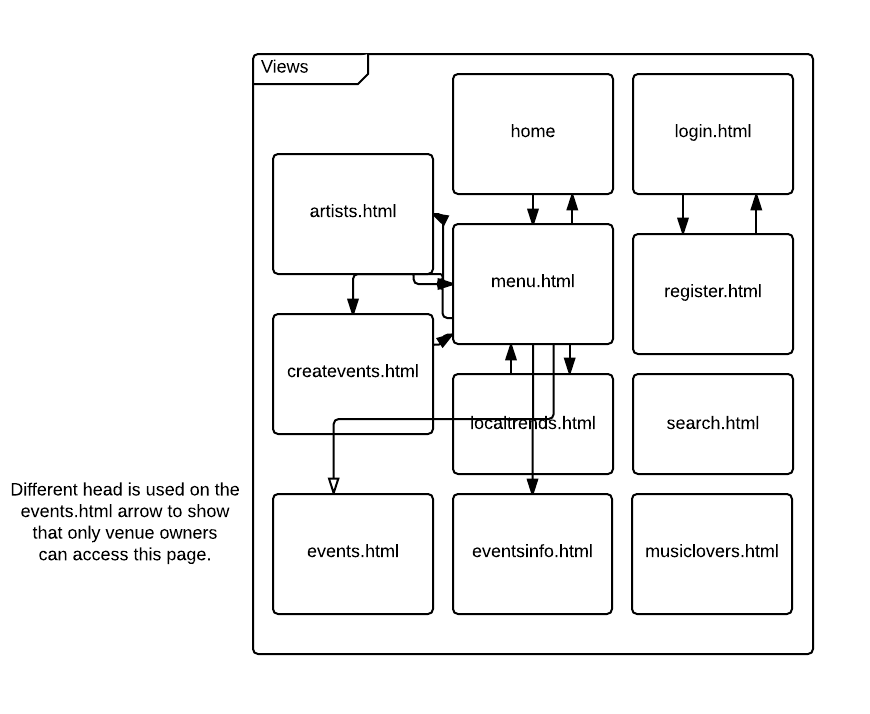
\includegraphics[width=\textwidth,height=\textheight,keepaspectratio]{images/va}
\caption{This UML diagram shows that once a user has logged in they can access multiple different pages through the menu bar (menu.html). The only page which is restricted is the events.html page as only venue owners can access this page to create events. The register.html page can only be accessed through the login page as it is accessed when a user needs to create a new account to login. UML diagram created using https://www.lucidchart.com/}
\end{figure}

\section{Some detailed design}
The following figure highlights the different relationships between the tables (model) for events.
\begin{figure}[H]
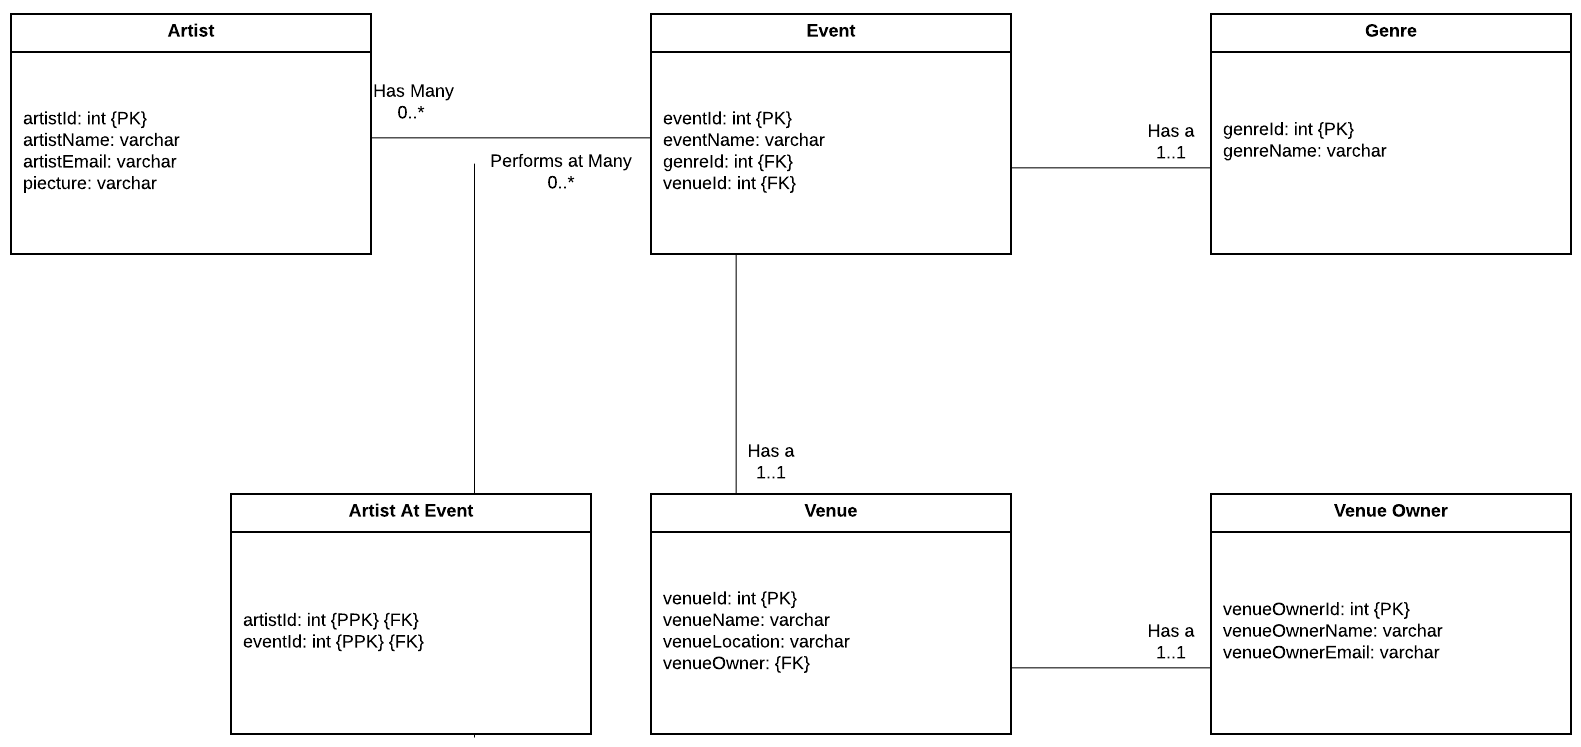
\includegraphics[width=\textwidth,height=\textheight,keepaspectratio]{images/events}
\caption{UML diagram which illustrates the appropriate relationships between the different tables in the database in relation to an event. Created using https://www.lucidchart.com/}

\end{figure}
\subsection{Even more detail}

\section{User Interface}

\section{Other relevant sections}